\chapter{Relevance to the Community}
\label{chapter:motivation}

\chapterprecishere{All of humanity's problems stem from man's inability to sit quietly in a room alone.\par\raggedleft--- \textup{Blaise Pascal}}
\chapterhung

In this chapter we present reasons why the community should find our challenges relevant and unveil requirements to avoid some of the problems.
We answer the research question:
\rqMotivation*

The chapter is structured as follows:

In \secref{observations} we discuss what we observed in FLOSS initiatives and companies.

In \secref{configuration-access} we conduct a study investigating the current state of configuration access.

In \secref{context-awareness} we discuss the current state of context awareness in FLOSS applications.

In \secref{configuration-challenges} we derive requirements from community feedback.






























\section{General Observations}
\label{sec:observations}

Because of the omnipresence of the configuration integration problem, developers invented many ad hoc solutions and workarounds.
The ad hoc solutions and workarounds are important puzzle pieces to understand the situation of the configuration integration problem.
The author of this book made many general observations during the years.
In this section we walk through important problems repeatedly found in many FLOSS initiatives and companies, answering the research question:
\rqMotivationObservation*

\subsection{Method}

We were involved in various FLOSS initiatives ourselves, for example, Performous (a karaoke application).
In this first section, we mainly rely on our own experience but we discussed the problems with experts, and other persons involved in FLOSS initiatives.

Personal observations and experience reports involve high subjectivity.
In particular, it is well-known that bias spreads across several cases.
If something is believed to be true because of multiple observations, it can be due to bias such as the illusory truth effect~\cite{hasher1977frequency}.
Because no findings here are inconsistent with other findings in the book, we likely forgot our wrong observations because of recall bias.
Unfortunately, knowing about a bias does not avoid having it.
Thus this material must always be considered critically and supplementary.

\subsection{Configuration Libraries}

From our experience FLOSS initiatives and companies tend to develop their own configuration libraries.
To make developers consider using existing configuration libraries, from the authors experience, it is essential that:

\begin{restatable}{requirement}{reqSimple}
A configuration library must be simple to use, easily available, light\-weight, efficient, and have an excellent out-of-the-box experience.%
\label{req:simple}
\end{restatable}

Often there are some constraints because of legacies, such as:

\begin{enumerate}
\item Customers already use legacy configuration file formats, and
\item it shall be possible to configure legacy software with the same configuration interfaces.
\end{enumerate}

\begin{restatable}{requirement}{reqLegacy}
A configuration library must be able to integrate (legacy) systems and must fully support (legacy) configuration files.%
\label{req:legacy}
\end{restatable}


\subsection{Duplication}

In larger applications duplicates related to configuration settings arise and have to be kept in sync.
Even in mature FLOSS initiatives, for example PostgreSQL---where the problem is already known and effort has been put into it---similar information needs to be synchronized in at least four places~\cite{online2016postgresql}.
Typically redundant, but with current approaches often unavoidable duplicates, are:

\begin{enumerate}
\item command-line interfaces (CLIs),
      graphical user interfaces (GUIs), and
      Web interfaces showing configuration settings,
\item command-line options and
      environment variables for overwriting a configuration setting,
\item validation code scattered and duplicated at several places,
\item several configuration files for different purposes\footnote{Such as configuration examples and default configuration files.},
\item test cases that run the application with different configuration settings,
\item documentation of the configuration settings, and
\item places where configuration settings are used within the application.
\end{enumerate}

The duplication makes it time-consuming to change, remove, or add existing configuration settings because always various places need to be considered.
Furthermore, the duplication makes it hard to get reliable information about configuration settings.

\begin{restatable}{requirement}{reqSpecification}
A single configuration specification must be able to include all information to generate all artifacts needed for configuration settings.
\end{restatable}

We saw several teams introducing their own identical configuration settings instead of sharing the configuration value of already given configuration settings.
This approach works nicely for the developers, who can avoid any collaboration and communication.
It creates, however, problems for system administrators who need to keep the duplicated configuration settings in sync.

\begin{restatable}{requirement}{reqSharing}
A configuration library must allow us to share configuration settings.%
\label{req:sharing}
\end{restatable}


\subsection{Inconsistencies}

Developers, maintainers, documentation writers, and system administrators easily create mismatches related to configuration settings.
In many cases this problem results from the duplication mentioned before.
We saw that:

\begin{itemize}
\item a configuration setting is misspelled at one of the duplicated places,
\item developers convert a configuration setting to a wrong type,
\item developers invent non-documented default value calculations and transformations,
\item the used configuration settings are not synchronized with the configuration settings of the configuration file,
\item data types or semantics of configuration settings differ between code and documentation, and
\item settings are hidden, i.\,e., used in the source but invisible otherwise.
System administrators do not know about such settings.
\end{itemize}

Of course, mismatches easily happen anywhere and anytime related to software.
The problem with configuration settings is that they cannot be tested exhaustively.
Testing is limited because all configuration settings can interact and create an exponential number of combinations.
In FLOSS software, often only the configuration settings as used by the (package) maintainer, developers, and testers are tested.
Thus system administrators have a good chance to find misbehavior if they facilitate rarely-used configuration settings.

\begin{restatable}{requirement}{reqGeneration}
The specification must enable code generation and inconsistencies must be ruled out during compilation.
\end{restatable}

For users and system administrators it is confusing if the configuration file has the correct content but applications do not use it.
For example, in a commercial application configuration settings only take effect after the next startup~\cite{jin2014configurations}.
We should avoid situations in which applications do not behave as their configuration files suggest:

\begin{restatable}{requirement}{reqConsistency}
\label{req:consistency}
Configuration libraries must provide ways to keep transient and persistent views consistent.
\end{restatable}

Users must be able to know which configuration settings exist, and which values are valid for them.
In case of doubt, it must be possible for system administrators to query which configuration settings and specifications are actually used:

\begin{restatable}{requirement}{reqIntrospection}
Configuration settings and specifications must be introspectable.%
\label{req:introspection}
\end{restatable}

\subsection{Maintenance}

As long as many similar and duplicated configuration settings exist, co-evolution is unavoidable.
It happens that:

\begin{itemize}
\item abundant code is accumulated around configuration accesses,
\item unused configuration settings are not visible and therefore cannot be cleaned up,
\item validation and transformation specifications need to be updated according to reported problems, and
\item outdated documentation for configuration settings needs to be corrected.
\end{itemize}

Such activities are time-consuming and error-prone, mainly because of the duplication.
Because these situations happen frequently, the source code likely gets inconsistent with the documentation.
Intensive testing would be needed but problems are often left for system administrators to find.

We found many workarounds because of bad API design.
In particular, in some applications we often found code that bypasses configuration access APIs.

\begin{restatable}{requirement}{reqMinimal}
The configuration access API must be minimal and crafted carefully.
\end{restatable}

A large technical debt is validation code spread over the whole source code.
We found that most of the code around configuration accesses tries to validate and transform configuration values.
This code was often executed much too late, causing hard-to-find misconfigurations.

\begin{restatable}{requirement}{reqValidate}
Validation of configuration settings must happen systematically before the application is even started.
\end{restatable}

We found complicated constructs that assign the return values of configuration accesses to variables.
Here people wanted to optimize the program and avoid calling configuration accesses within loops.

\begin{restatable}{requirement}{reqFast}
Developers must have guarantees that read-only configuration access is fast and updates only happen if wanted.%
\label{req:fast}
\end{restatable}

\subsection{Result}

Here we answer the research question:
\rqMotivationObservation*

\begin{finding}
Due to observations we found that many small duplications of configuration settings and specifications lead to inconsistencies and increase maintenance costs.
\end{finding}

We have listed requirements that intend to reduce these problems.

















\section{Current State of Configuration Access}
\label{sec:configuration-access}

For the book we want to focus on configuration access that is indeed relevant and popular.
In this section we investigate which kind of configuration access FLOSS developers prefer and how configuration access is currently done, answering the research question:
\rqMotivationCurrentState*

\subsection{Method}
\label{sec:motivation-method}

In the main part of this section, we use labels to indicate which method we used.
The label ``\methodQuestion{}'' (without quotes) indicates that data was collected from the questionnaire survey and the label ``\methodSource{}'' (without quotes) represents that data was gathered from the source code analysis.

\subsubsection{Questionnaire (Label \methodQuestion{})}

The author of the book formulated questions with FLOSS developers as main target.
Three students added some questions for their bachelor book.
They created two questionnaires using LimeSurvey and Google Forms.
Then we organized several pilot surveys with colleagues, FLOSS developers, and experts for surveys.
Based on the feedback, we decided to use LimeSurvey and improved the questions, answers, and visual appearance~\cite{raab2017challenges}.

To be sure that we reach our main target group, we posted requests for participation in many relevant FLOSS communication channels.
We rewarded non-anonymous answers by donations to initiatives related to FLOSS.
For quality assurance, we cross-checked these non-anonymous answers with the complete pool of participants~\cite{raab2017challenges}.
The survey was reachable from \formatdate{20}{6}{2016} to \formatdate{18}{7}{2016}.
After the survey was completed, we sent an email to all non-anonymous participants.

LimeSurvey version 2.50+ aided us for conducting the survey.
The questionnaire started with an introduction and personal questions to have characteristics of our group.
The personal questions included education, occupation, age, and FLOSS participation~\cite{raab2017challenges}.
We did not ask any gender-related questions because we did not expect enough participation for significant conclusions.
The main part consisted of questions about why and how developers use configuration.
We added open questions at the end of the questionnaire for a qualitative touch.

In this book original questions are written down using the format \question{Original question}.
We report the percentages relative to the number of participants~($n$) answering the particular question.
We note standard deviations ($s$) and means for samples of $n\geq95$.
We utilized the Kolmogorov-Smirnov test~\cite{lilliefors1967kolmogorov} for samples of smaller size~\cite{raab2017challenges}.

\subsubsection{Source Code Analysis (Label \methodSource{})}

Different from earlier work~\cite{xu2013blame,zhang2014configuration,keller2008conferr,jin2014configurations}, we do not want to limit ourselves to configuration files.
Instead we extend our studies to ^getenv^, which is a configuration access API to query \empha[environment variable]{environment variables}.
We chose it because it is unique in its availability\footnote{It is readily available in nearly all programming languages, for example, it is included in the standard libraries of Java, C, C++, Python, Lua, and many more.} and standardization\footnote{It is standardized by SVr4, POSIX.1-2001, 4.3BSD, C89, and C99~\cite{man2017getenv}.}~\cite{raab2017challenges}.

\begin{table}[htp]
\begin{tabularx}{\columnwidth}{l  R |  l R}
\toprule
{\bfseries Application} &
{Version} &
{\bfseries Application} &
{Version}
\\
\hline


0ad & 0.0.17                           &          Gimp & 2.8.14\\
Akonadi & 1.13.0                       &          Inkscape & 0.48.5\\
Chromium & 45.0.2454                   &          Ipe & 7.1.4\\
Curl & 7.38.0                          &          LibreOffice & 4.3.3\\
Eclipse & 3.8.1                        &          Lynx & 2.8.9dev1\\
Evolution & 3.12.9                     &          Man & 2.7.0.2\\
Firefox & 38.3.0esr                    &          Smplayer & 14.9.0\~{}ds0\\
GCC & 4.9.2                            &          Wget & 1.16\\

\hline

\bottomrule

\end{tabularx}
\caption{Versions of applications studied.}
\label{tab:versions}
\end{table}

We analyze the usage of the function ^getenv^ in the source code.
We carefully elected 16 FLOSS applications across different domains such as desktop, development, mobile, games, and system utilities.
Our selection criteria were popularity, code size, and a thriving community.
We included individual other applications for diversity.
As shown in \tabref{versions}, we consistently used the versions as part of Debian GNU/Linux 8 (Jessie)~\cite{raab2017challenges}.


We downloaded packages with ^apt-get source^ from \url{http://snapshot.debian.org}~\cite{raab2017challenges}.
To determine the code size we facilitated Cloc 1.60~\cite{danial2017cloc}.

We wanted to know how many of the textual ^getenv^ occurrences are  real ^getenv^ invocations, i.\,e.\ configuration access points, as opposed to occurrences in comments etc.
Thus we counted them manually for the versions as specified in \tabref{versions}~\cite{raab2017challenges}.
Obvious wrapper functions that include ^getenv^ within their name are evaluated identically to ^getenv^ itself~\cite{raab2017introducing}.
We excluded some ^getenv^ occurrences:
\begin{itemize}
\item
We did so if the ^getenv^ invocation is obviously related to debugging, logging and testing.
Such situations were determined by looking at the ^getenv^ parameter.
\item
We did so if the ^getenv^ invocation is obviously related to the build system, and not used in the application.
\end{itemize}
The rationale behind these exclusions is that our study should be generalizable to run-time configuration access, and not be specific to ^getenv^.

\subsubsection{History Analysis}

For the analyses of the histories we looked at the same applications as specified in \tabref{versions}.
We used Git repositories, even if the official repository used a different version control.
Because of the immense number of commits in the application's repositories, we could not use Cloc for the histories\footnote{It took weeks to run through all commits even without Cloc.}.
Manually counting ^getenv^ in every commit was also out of question.
Therefore, we used the line-counting tool ^wc -l^ and ^grep -rio getenv^ (with binary and project files filtered out).




\subsection{Threats to Validity}
\label{sec:motivation-threats}

As proposed by mixed methods, the combination of different analyses returns a more complete picture~\cite{ihantola2011threats}.
Nevertheless, each of the individual methods needs to be conducted with great care.
Threats to validity concern the questionnaire, the source code analysis, and the history analysis.
Here we describe our mitigation strategies categorized by these methods.%
{\parfillskip=0pt plus .7\textwidth \emergencystretch=.5\textwidth \par}

\subsubsection{Questionnaire (Label \methodQuestion{})}

Surveys reflect beliefs and wishful thinking of participants.
Hence, we cross-checked with other methods for facts in the source code of the applications.
Nevertheless, opinions assist in understanding reasons and goals, thus the survey is an essential part of the overall work.
We consider it as important supplement to source code analysis~\cite{raab2017challenges}.

For the questionnaire survey's validity we had to make sure that only FLOSS contributors participate.
To mitigate this threat~\cite{raab2017challenges}:
\begin{itemize}
\item We made clear in the introduction that the study is related to FLOSS, by starting with
\question{This survey targets developers of free and open source software (FLOSS) applications}.
\item We prompted the participants about involvement in FLOSS initiatives.
\item We invited persons via communication channels that are most likely read by FLOSS contributors.
\item We advertised with donations to FLOSS initiatives.
\end{itemize}

Anonymized raw data for better reproducibility and the questions in full for better repeatability are found at~\cite{raab2017challenges,vitek2011repeatability,blackburn2016truth}:
\par \hspace{12em}\url{https://rawdata.libelektra.org}. \par

\subsubsection{Source Code Analysis (Label \methodSource{})}

Manual analysis has the danger of oversight and subjective classification.
To minimize such errors we incorporated second opinions and only report large differences~\cite{raab2017introducing}.

An important matter is whether the applications and their developers are representative.
We address it by studying 16 mostly diverse applications.
We added both large and small applications.
We took care that various development teams, domains, and programming languages are represented.
The browsers are also used in mobile contexts~\cite{raab2017introducing}.

We have to acknowledge that the majority of evaluated software is implemented in C/C++.
Nevertheless, Java, JavaScript and Python are represented with 4.3, 3.3, and 1.1 million lines of code, respectively.
Furthermore, we included Eclipse to have a huge FLOSS initiative mainly implemented in Java~\cite{raab2017introducing}.

An equally important threat to validity is whether ^getenv^, our prime subject of study, represents configuration access points in general.
According to previous studies~\cite{jin2014configurations,rabkin2011static,xu2013blame}, configuration access points are in their essence simple key-value accesses.
Higher-level configuration accesses, for example with complex data types, would only complicate the implementation of the configuration access APIs~\cite{behrang2015users,raab2017introducing}.

Some FLOSS initiatives contain ^getenv^ invocations in scripts used to configure their compilation.
These invocations are not part of the final executable and are irrelevant for our goal of making software context aware at run-time.
We did not include such invocations to ^getenv^ in our classification.
It is not always easy to tell which parts of the source code actually end up in a given binary.
We might have included some ^getenv^ invocations in the analysis that are actually not included in the executable of the application.
Thus we might slightly overestimate the number of ^getenv^ occurrences.

Because we conducted a source code analysis, we were not able to pick closed-source applications.
A portion of the evaluated software, however, has its roots as closed-source applications.
Also based on our experience within companies, we are confident that our conclusions hold for closed-source applications, too~\cite{raab2017introducing}.


\subsubsection{History Analysis}

Some applications did not have a linear history.
In some cases, different repositories without common ancestors were merged.
Even though we worked with great care, it is possible that we did not always pick the right commits.
If this often happened, we might have missed trends that are there.


\subsection{Configuration Access in FLOSS}

\subsubsection{What was the population of the survey?}

\methodQuestion{}
From 672 persons visiting the survey 286 started to answer.
From them, 162 persons completed the questionnaire and 116 persons left their email address.

The age of the population ($n=220$) has a mean of 32 years ($s=9$, \question{How old are you?}).
As occupation, \p{56} of the persons selected software developer, \p{21} system administrator, and \p{16} researcher (multiple choice question, $n=287$, \question{What is your occupation?}).
The participants ($n=242$, \question{Which country are you from?}) said they are from Germany (50), Austria (41), United States (32), France (25), Australia (9), and 31 other countries (85).
The reported degrees of the persons ($n=244$, \question{Which is the highest degree that you have?}) are: master (\p{38}), bachelor (\p{25}), student (\p{18}), no degree (\p{13}), and PhD (\p{6}).

In the questionnaire we asked to fill out information for up to five different FLOSS initiatives (\question{In which free and open source software (FLOSS) projects have you been or are you involved?}).
For the first FLOSS initiatives, persons estimated their participation time with a mean of 5.3 years ($s=5$, $n=180$, \question{Length of Participation [years]}).
Of these persons, \p{60} reported a second FLOSS initiative, \p{36} a third, \p{17} a fourth, and \p{9} a fifth.
All persons together reported that they participated in 400 FLOSS initiatives, from which 282 were unique\footnote{With normalized names and collapsed ``various'' and ``personal'' FLOSS initiatives.}.
Debian was the most often mentioned initiative (28), then GNOME and KDE (9), and then Linux (7).



\subsubsection{Which methods for configuration access are popular?}
\label{survey}

\begin{finding}
Command-line arguments, environment variables, and configuration files are equally popular.
Developers are very satisfied with them.
Other configuration accesses are less popular---both in reported use and satisfaction~\cite{raab2017challenges}.
\end{finding}

The finding leads to the requirement:

\begin{restatable}{requirement}{reqEnvironment}
A configuration library must support all three popular ways for configuration access:
configuration files, command-line options, and environment variables.
\end{restatable}

\methodQuestion{}
Command-line arguments (\p{92}, $n=222$), environment variables, for example, via ^getenv^ (\p{79}, $n=218$), and configuration files (\p{74}, $n=218$) are the most popular ways to work with configuration settings (\question{Which configuration systems/libraries/APIs have you already used or would like to use in one of your FLOSS project(s)?}).%
{\parfillskip=0pt plus .7\textwidth \emergencystretch=.1\textwidth \par}

Others---namely X/Q/GSettings (\p{4}, \p{11}, \p{9}), KConfig (\p{5}), dconf (\p{7}), plist (\p{7}), and Windows Registry (\p{13})---were used less ($\leq$ \p{13}, $n\geq185$). %win reg used most
Freedesktop standards' usage, for example shared-mime-info, is in between (\p{20}, $n=205$).

Persons seldom found it (very) frustrating to work with the popular systems (\question{What is your experience with the following configuration systems/libraries/APIs?}):
^getenv^ (\p{10}, $n=198$), configuration files (\p{6}, $n=190$), and command-line options (\p{4}, $n=210$).
Less-used systems frustrated more ($\geq$ \p{14}, $n\geq 27$):
X/Q/GSettings (\p{41}, \p{14}, \p{35}), KConfig (\p{21}), dconf (\p{42}), plist (\p{32}), or Windows Registry (\p{69}).
QSettings is the most popular API from the lesser-used ones with \p{51} of (very) satisfied users.%
{\parfillskip=0pt \emergencystretch=.5\textwidth \par}

\begin{finding}
The API \texttt{getenv} is used omnipresently with 2,683 occurrences.
\end{finding}

\methodSource{}
\tabref{lines} shows the number of occurrences of ^getenv^ per application as we counted them manually.%
{\parfillskip=0pt plus .7\textwidth \emergencystretch=.2\textwidth \par}

\begin{table}[htp]
\begin{tabularx}{\columnwidth}{l  R  R  R}
\toprule
\multicolumn{1}{l}{\bfseries Application} &
\multicolumn{1}{R}{\bfseries \blap{1k lines\\of code}} &
\multicolumn{1}{R}{\bfseries \blap{counted \\ \texttt{getenv}}} &
\multicolumn{1}{R}{\bfseries \blap{lines per\\ \texttt{getenv}}}
\\
\hline

0ad 		&	474   	&	55 	&	8,617  \\
Akonadi 	&	37    	&	13 	&	2,863  \\
Chromium 	&	18,032	&	770	&	23,418 \\
Curl 		&	249    	&	53 	&	4,705  \\
Eclipse 	&	3,312 	&	40 	&	82,793 \\
Evolution 	&	673   	&	23 	&	29,252 \\
GCC 		&	6,851 	&	377	&	18,172 \\
Firefox 	&	12,395	&	788	&	15,730 \\
Gimp 		&	902   	&	56 	&	16,102 \\
Inkscape 	&	480   	&	19 	&	25,255 \\
Ipe 		&	116   	&	21 	&	5,529  \\
LibreOffice 	&	5,482 	&	284	&	19,304 \\
Lynx 		&	192   	&	89 	&	2,157  \\
Man 		&	142   	&	62 	&	2,293  \\
Smplayer 	&	76   	&	1  	&	76,170 \\
Wget 		&	143   	&	32 	&	4,456  \\
\hline
Total	&	49,556	&	2,683	&	18,470 \\
Median	&	477	&	54	&	       \\

\bottomrule
\end{tabularx}
\caption[Manually counted \texttt{getenv}.]{Manually counted \texttt{getenv}~\cite{raab2017introducing}:
The column \emph{1k lines of code} are the lines of codes of the applications divided with a factor of 1,000.
The column \emph{counted \texttt{getenv}} contains our manual count of \texttt{getenv} invocations.
The column \emph{lines per \texttt{getenv}} is the ratio of the lines of code and manually counted \texttt{getenv}.
}
\label{tab:lines}
\end{table}





\subsubsection{Why are currently so many configuration file formats present?}

\begin{finding}
New configuration file formats were introduced by \p{19} of the persons.
\end{finding}

\label{res:invented-configuration-file-format}
\methodQuestion{}
The \p{19} persons ($n=251$, \question{In which way have you used or contributed to the configuration system/library/API in your previously mentioned FLOSS project(s)?}), who claim to have introduced a configuration file format, confirm that regularly many new configuration file formats get invented.
Furthermore, \p{29} implemented a configuration file parser.
Fewer persons (\p{15}) introduced a configuration system/library/API.
Using internal (\p{35}) and external configuration access APIs (\p{34}) is more popular than reinventing new formats or APIs.

\paragraph{Discussion:}
More configuration file formats are invented (\p{19}) than configuration system/library/API(s) introduced (\p{15}).
This suggests that many configuration file formats do not have a proper library/API for them.







\subsection{Purpose and Trend of \texttt{getenv}}

\subsubsection{What is the purpose of \texttt{getenv}?}

\begin{finding}
\label{fnd:getenv-configuration}
In most aspects ^getenv^ has the same purpose as other configuration access APIs.
Specific to ^getenv^ is its utilization for:
\begin{enumerate}
\item bypassing other configuration accesses (\methodQuestion{} \p{45}),
\item locating configuration files,
\item debugging and testing (\methodQuestion{} \p{55}, \methodSource{} 1,152, i.\,e. \p{43}), and
\item sharing configuration settings across applications (\methodQuestion{} \p{53}, \methodSource{} 716, i.\,e. \p{47}).
\end{enumerate}
\end{finding}

Item~4 of this finding is an indication that there is a need for our Requirement~\reqref{sharing}:
\reqSharing*


\methodQuestion{}
In a multiple choice question we found that the reasons to use ^getenv^ vary ($n=177$, \question{At which places in the code would you use a \texttt{getenv}?}):
\begin{description}
\item[\p{55}] say they would use it for debugging and testing,
\item[\p{53}] say they would use it for configuration integration, i.\,e., sharing configuration settings (answer ``environment variables'' from question \question{Which effort do you think is worthwhile for providing better configuration experience?}),
\item[\p{45}] would use ^getenv^ to bypass the application's main configuration access,
\item[\p{20}] would use ^getenv^ if they consider configuration settings unlikely to be changed by a user, and
\item[\p{2}] say they would use ^getenv^ in a loop (\question{even when it is used inside a loop, for example: \lstinline[language=Cpp]^for (int i = 0; i < K; ++i) getenv("HOME");^}).
\end{description}

\methodSource{}
Out of the 2,683 ^getenv^ invocations, we classified 1,531 ^getenv^ invocations, i.\,e.\ \p{57}, not to be used for logging, debugging, testing, or similar.
By analyzing which parameters are passed to non-testing ^getenv^ invocations we found 716 invocations (\p{47}) using shareable parameters, such as ^PATH^.

As mentioned in the method section, we separated the ^getenv^ invocations for debugging and testing because we wanted to avoid that our results are specific to ^getenv^.
Configuration settings in configuration files usually do not have so many settings dedicated to debugging and testing.
Thus further investigations in this book elaborate exclusively on these 1,531 ^getenv^ invocations.


\begin{table}[htp]
\begin{tabularx}{\columnwidth}{l  R  R | l R  R}
\toprule
{\bfseries Application} &
{\bfseries conf} &
{\bfseries uniq} &
{\bfseries Application} &
{\bfseries conf} &
{\bfseries uniq}
\\
\hline

0ad 		&    45  &    25   &Gimp 		&    27  &    22   \\
Akonadi 	&    8   &    5    &Inkscape	&    16  &    11   \\
Chromium 	&    387 &    234  &Ipe 		&    19  &    12   \\
Curl 		&    26  &    20   &LibreOffice 	&    207 &    120  \\
Eclipse 	&    33  &    24   &Lynx 		&    79  &    53   \\
Evolution 	&    13  &    11   &Man 		&    52  &    35   \\
GCC 		&    218 &    127  &Smplayer	&    1   &    1    \\
Firefox 	&    376 &    245  &Wget 		&    24  &    17   \\

\hline
\bottomrule

\end{tabularx}
\caption{Counted number of \texttt{getenv} invocations without debugging and testing.}
\label{tab:countconf}
\end{table}

\methodSource{}
\tabref{countconf} presents the results of the classification.
The column \emph{conf} shows the number of ^getenv^ invocations broken down from the before-mentioned 1,531 ^getenv^ invocations.
The column \emph{uniq} displays how many of them had different parameters.

Most ^getenv^ invocations pass a string parameter defined nearby in the source code (\p{95}).
Only in 71 cases it was unclear which string is passed to the ^getenv^ invocation.

\paragraph{Analysis of \texttt{getenv} parameters:} 357 configuration access points (105 unique) manage configurable file system locations, for example, download directories or paths to configuration files. % "PATH\^HOME\^DIR"
Some configuration access points configure the user interface, such as whether native widgets shall be used, for example, ^AQUA_NATIVE_MENUS^.
Furthermore, 97 configuration access points (15 unique) configure the language, for example, ^LANG^. % "CHARSET\^LANG\^LC" ^ grep -v "TOOLCHAIN\^CLANG\^CLASS\^OPENCL\^CLCOPY"
Some applications have a large amount of application-specific parameters to ^getenv^, for example, Firefox has 117 configuration access points (89 unique) with ^MOZ_*^ or ^GECKO_*^ as parameters. %"MOZ\^GECKO"
Some parameters ensure compatibility with previous or standard behavior, for example ^POSIXLY_CORRECT^.
Other parameters probe hardware, for example, 58 parameters (42 unique) probe OpenGL support.
For common parameters, we found different spellings or capitalizations, for example, ^TMP^, ^TEMP^, or ^TMPDIR^.

We found configuration accesses that were outdated and not used anymore.
We wrote 4 bug reports, 2 of them were acknowledged and 1 was fixed.\footnote{Reported by us in \url{https://savannah.gnu.org/bugs/index.php?47989}.}

\paragraph{Discussion:}
Overall we found the characteristics of ^getenv^ parameters to be very similar to other configuration accesses like configuration settings in configuration files.
One special property of ^getenv^ is that parameters are commonly shared between applications (such as ^PATH^) but with some fragmentation.
The analysis of the ^getenv^ invocations surprised us by very different uses:
In some cases, environment variables are misused as global variables.
Some ^getenv^ invocations obviously bypass the application's main configuration access.
We found different reasons for bypasses:
\begin{itemize}
\item To locate the configuration files avoiding otherwise necessary \empha{bootstrap} code.
\item Because ^getenv^ was more readily available, for example, a pointer to the data structure of main configuration access was missing at that place.
\item It was added temporarily but never removed.
\end{itemize}


\subsubsection{What is the trend of \texttt{getenv} occurrences?}

\begin{finding}
In an analysis of the development histories of the 16 applications we observed that \texttt{getenv} occurrences rarely decrease.
\end{finding}

\figref{history} shows the historical development of textual ^getenv^ occurrences and the textual lines in the repositories for Firefox and Chromium.

\begin{figure}[htp]
\centering
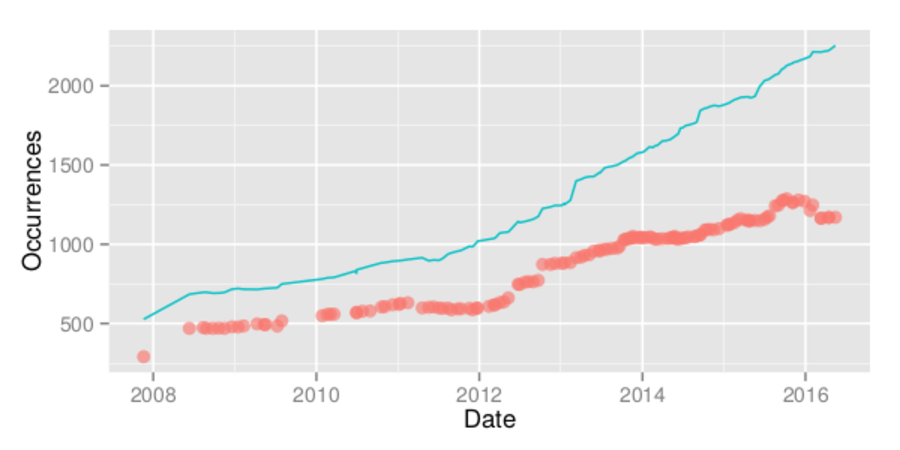
\includegraphics[scale=0.7]{firefox}
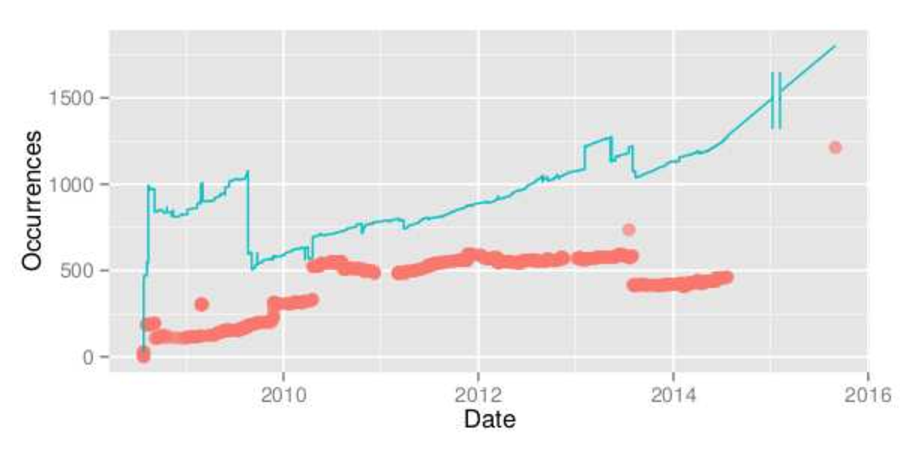
\includegraphics[scale=0.7]{chromium}
\caption[History of getenv occurrences.]{The red points show occurrences of the text \texttt{getenv} in the repository of Firefox (above) and Chromium (below).
We suppress points where the number has not changed between commits.
The continuous, thin line indicates total lines of the application's source code.
They are counted with \texttt{wc} and expressed as multiples of \emph{10,000}.
The repository contains files not present in the Debian source package we analyzed.
The \emph{date} dimension goes beyond the release date of the manually evaluated Firefox version (\formatdate{22}{9}{2015}).
In Chromium, we added the manually evaluated version.
The graphs are representative for about half of the evaluated software, others are highly irregular.%
{\parfillskip=0pt plus .8\textwidth \emergencystretch=.5\textwidth \par}}
\label{fig:history}
\end{figure}

\begin{implication}
This inflation indicates research on ^getenv^ is future-proof and system administrators may get even more complex interfaces in the future.
\end{implication}




\subsubsection{How are \texttt{getenv} parameters documented?}

\begin{finding}
The documentation of \texttt{getenv} parameters is not satisfactory.
\end{finding}

\paragraph{Method:}
Using \url{startpage.com} we searched for every parameter passed to ^getenv^ invocations.
If there were too many results, we added the name of the application.
We did not look at the second page, i.\,e., we only investigated the first ten links.

\paragraph{Result:}
\methodSource{}
For only $283$ non-shared ^getenv^ parameters we found documentation.
We could not find explanations of the behavior of the $387$ other ^getenv^ parameters~\cite{raab2017challenges}.

\paragraph{Discussion:}
We found different ways how FLOSS initiatives deal with lacking documentation of ^getenv^ parameters.
Many FLOSS initiatives declare ^getenv^ use as internal:
They officially do not recommend using them, even if no other workaround exists.
Such statements contradict our finding that only \p{20} of FLOSS developers consider environment variables unlikely to be changed.
In some FLOSS initiatives the contributors compile lists of available parameters.
For example, LibreOffice contributors find ^getenv^ invocations with ^grep^\footnote{Which has limitations regarding \texttt{getenv} aliases and is also not intended for users, see \url{https://bugs.documentfoundation.org/show_bug.cgi?id=37338}.}~\cite{raab2017challenges}.



\subsection{Result}

Here we summarize our results for the research question:
\rqMotivationCurrentState*

\begin{finding}
We found that three types of execution environments are especially popular:
configuration files, environment variables, and command-line options.

We unveiled details about why it is often arbitrary which of the execution environments is chosen:
\begin{itemize}
\item Often the most convenient method is used.
\item In the survey, people often could not agree what ^getenv^ shall be used for (Most results are around \p{50}.)
\end{itemize}
\end{finding}

The ^getenv^ API supports all characteristics for configuration access and can be used to investigate challenges in configuration validation.

Environment variables cannot replace configuration files because they do not support to be persisted or to be changed from outside during execution.




































































\section{Current State of Context Awareness}
\label{sec:context-awareness}

In this section we answer the research question:
\rqMotivationContext*

\begin{hypothesis}[RQ~\ref{rq:motivation-context}]
We expect at least some configuration accesses to be context unaware as candidates for improvements.
\end{hypothesis}


\rqsubsection{motivation-context-usage}{What are the usage patterns of \texttt{getenv}?}
\label{sec:context-context-usage}

In this part we investigate if configuration access points already consider context.
We focus on the configuration access points using the API ^getenv^.

\subsubsection{Method}

We refined our classification by determining whether ^getenv^ invocations for configuration \emph{provide} or \emph{require} configuration context.
We say that some configuration access code \emph{requires context} if it is executed conditionally depending on some configuration value.
The configuration access code controlling such conditional branches is said to \emph{provide context} for the conditionally executed code.

\begin{example}
Consider the following code snippet adapted from Lynx:

\begin{code}[language=Cpp]
if (lynx_cfg_file == NULL) {
   if ((cp = getenv ("LYNX_CFG")) != NULL)
       lynx_cfg_file = strdup (cp);
}
\end{code}

Here the ^getenv^ invocation \emph{requires} configuration context:
It is conditionally executed depending on the existence of a configuration file in a place that may have been configured by a command-line option.
This ^getenv^ invocation \emph{provides} context for further configuration access code because it controls where configuration settings will be searched.
\end{example}

We only looked at code snippets with 20 surrounding code lines.
In some cases this made it difficult to judge whether a ^getenv^ invocation needed or provided context.
In such cases we were conservative and did not count the invocation as needing or providing context, except for invocations which are presumably used to locate configuration files.
Our results may be skewed by the fact that some FLOSS initiatives include source code from others.
For example, Chromium and Firefox both include source code of the SQLite library that contains ^getenv^ invocations.
Chromium even contain two slightly different versions of at least some of this code.

Then we tagged contexts of configuration access points into categories.
The categories classify the purpose of the context, for example, \lstinline[language=Cpp]^if (running_os_X) getenv(..);^ is in the ^os_X^ category.


\subsubsection{Result}

As shown in Figure~\ref{fig:np} we identified 837 configuration access points where context is needed.
We found 750 places where the return value of ^getenv^ provides context for configuration related code.

\begin{figure}[htp]
\centering
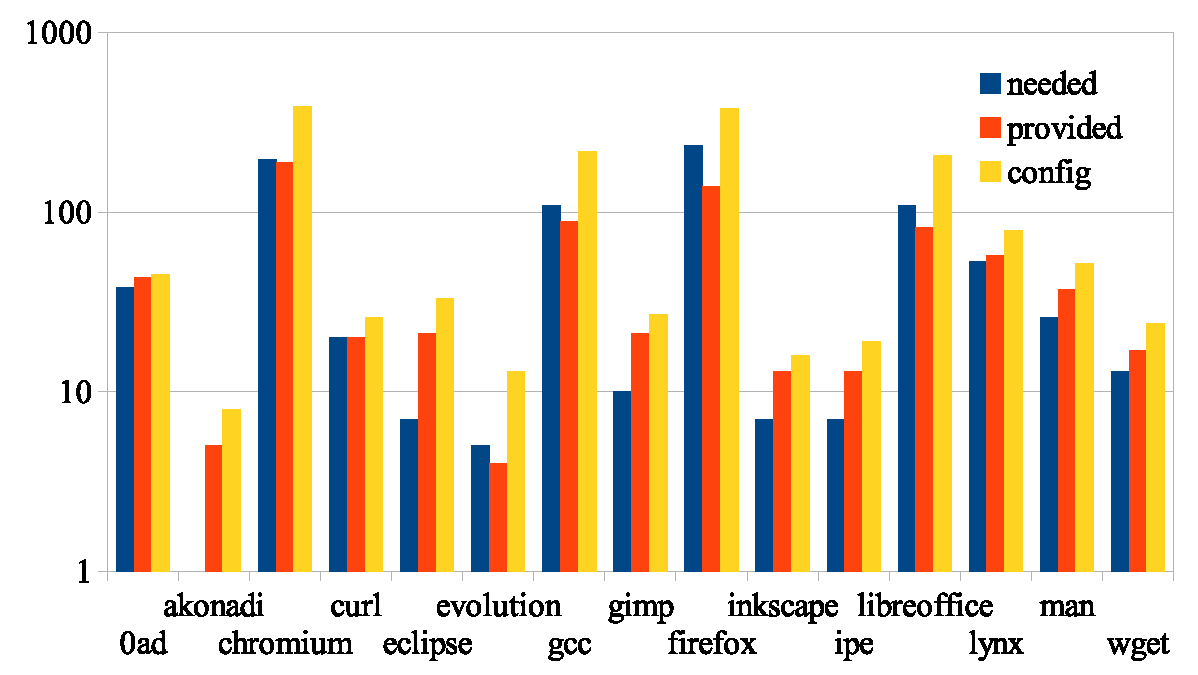
\includegraphics[width=\columnwidth]{npc}
\caption[Classification of needed and provided contexts.]{%
Classification of \emph{needed} and \emph{provided} contexts per application with a logarithmic scale;
\emph{config} is the number of configuration-related configuration access points (in total 1,531).}
\label{fig:np}

\end{figure}

We introduced 152 categories of contexts.
The categories include operating systems ^os_*^, ^getenv^ invocations ^getenv_*^, locales, network, cmdline, build system, debug, hardware specifics ^hw_*^, system specifics ^sys_*^, file system paths ^path_*^, and others.
Developers put by far the greatest effort into correctly handling the context the operating system provides.
They considered 36 different operating systems, with most occurrences for different versions of Windows (155), various UNIX clones (127), Android (59), and VMS (23).%
{\parfillskip=0pt \emergencystretch=.5\textwidth \par}

We found 102 invocations to ^getenv^ depend on other invocations to ^getenv^, often because of fallback chains that support similarly named settings (for example, ^TMP^, ^TEMP^, or ^TMPDIR^).
Hardware-based features were not often used as context but they were diverse, for example, configuration access points checking for AES or SSE instruction set features.
In 38 places the name or presence of files formed a context.
Many contexts occurred only for a single configuration access point, for example, a specific software dependence.%
{\parfillskip=0pt \emergencystretch=.5\textwidth \par}

\subsubsection{Discussion}

We searched for places where more context would be useful.
Here, by nature, subjectivity is involved.
We only report the numbers we found but avoid building any finding or implications on the number.
We found 129 such places, with complaints on the Internet in 23 cases.

We answer the research question:
\rqMotivationContextUsage*

\begin{finding}
Source code to consider context often occurs around configuration access points.
We found 837 configuration access points where context is manually considered, and 750 configuration access points that provide context for others.
Developers focus on support for various operating systems.
It is inevitable that in many places the context is forgotten:
we found cases with complaints in the Internet.

\begin{implication}
Based on the 837 needed and 750 provided contexts around configuration access points, we assume developers tried hard to support context awareness.
\end{implication}
\end{finding}








\rqsubsection{motivation-context-repeat}{How often is \texttt{getenv} repeatedly used at run-time?}

As we learned from the questionnaire survey, nearly no developer thought ^getenv^ should be used in a loop.
Therefore, if ^getenv^ is nevertheless repeatedly invoked with the same parameters, it is possible that developers assumed different semantics than ^getenv^ actually has:
All ^getenv^ calls within the process return a value initialized at application's start.
Thus ^getenv^ return possibly-outdated, non-context-aware values repeatedly, which is a lost opportunity for better context awareness.



\subsubsection{Method}

To improve reproducibility we freshly installed Debian GNU/Linux Jessie with KDE and GNOME desktop, respectively.
Only one measurement (of the boot up) was done with the GNOME variant.
We applied only small modifications after the fresh installation:
We installed the mentioned applications\footnote{If not already part of the default installation.} and \elektra{}~\cite{raab2016unanticipated}.
Furthermore, we configured Akonadi to use an IMAP account.


For more accurate interpretation of the numbers it is important to know that usage patterns vary widely between different hardware, operating systems, and installed packages.
For example, Firefox executed within GNOME\footnote{Which was not used in the main experiment.} triggered 11 GNOME-specific and 8 GTK-specific ^getenv^ invocations~\cite{raab2016unanticipated}.
In the KDE desktop, these ^getenv^ invocations would not occur.
The differences caused by the environment are drastic.
For example, on the author's laptop EliteByte (running KDE with many additionally installed applications), we counted 210.276 ^getenv^ invocations during startup.
This number is 21 times more than the number counted on a freshly installed KDE.


We examine how applications use ^getenv^ repeatedly.
Only APIs that are repeatedly used at run-time flawlessly support context awareness.
To learn about usage patterns of ^getenv^, we count executions of ^getenv^ by logging all invocations~\cite{raab2016unanticipated}.




\subsubsection{Result}

{
\setlength{\arrayrulewidth}{.08em} 
\begin{table}[htp]
\begin{tabularx}{\textwidth}{ l  r  R  R  R  R  R   }
\toprule
\multicolumn{1}{l}{\bfseries Application} &
\multicolumn{1}{R}{\bfseries \shortstack{lines of\\ code}} &
\multicolumn{1}{R}{\bfseries \shortstack{\texttt{getenv} \\ all}} &
\multicolumn{1}{R}{\bfseries \shortstack{\texttt{getenv} \\ init}} &
\multicolumn{1}{R}{\bfseries \shortstack{all \\ unique}} &
\multicolumn{1}{R}{\bfseries \shortstack{later \\ unique}} &
\multicolumn{1}{R}{\bfseries \shortstack{ \\  same}}
\\
\hline
Akonadi & 37,214      & 10,357 & 8655 & 110 & 12 &    5126  \\
Chromium & 18,032,183  & 6006 & 1803 & 1118 & 192 &     165  \\
Curl & 249,380        & 19 & 8 & 12 & 8 &       4  \\
Eclipse & 3,311,712    & 2790 & 2696 & 389 & 42 &    1495  \\
Evolution & 672,789   & 4407 & 1488 & 1060 & 24 &     163  \\
Firefox & 12,394,938   & 3371 & 2049 & 276 & 70 &     895  \\
Gimp & 901,703        & 2551 & 1115 & 217 & 137 &     364  \\
Inkscape & 479,849    & 722 & 457 & 160 & 51 &     166  \\
LibreOffice & 5,482,215& 3354 & 2891 & 258 & 59 &    1493  \\
Lynx & 192,012        & 1931 & 961 & 27 & 27 &     923  \\
Man & 142,183         & 2862 & 13 & 86 & 76 &       2  \\
Smplayer & 76,170     & 212 & 164 & 71 & 8 &      53  \\
Wget & 142,603        & 11 & 10 & 8 & 1 &       3  \\


\hline
Median       & 479,849 & 2790 & 1115 & 160 & 42 & 166 \\
Total        & 41,821,956 & 38,593 & 22,310 & 3792 & 707 & 10,852 \\



\hline
KDE          & * & * & 9606 & 265 & * & 2634 \\
GNOME        & * & * & 144  & 47 & *  & 4 \\



Debian       & * & * & 5317 & 430 & * & 286  \\



\end{tabularx}
\caption[Count of \texttt{getenv} at run-time.]{Count of \texttt{getenv} during run-time. The star (*) means that any of the above applications can be started in the session~\cite{raab2016unanticipated}.}
\label{tab:count-runtime}
\end{table}
}

In \tabref{count-runtime} we use the following columns~\cite{raab2016unanticipated}:
\begin{description}
\item[lines of code:] Counted lines of code.
\item[\texttt{getenv} all:] Counted ^getenv^ invocations while using the applications.
\item[\texttt{getenv} init:] Counted ^getenv^ invocation while starting up the applications.
\item[all unique:] From \emph{\texttt{getenv} all}: How many different parameters were used?
\item[later unique:] From ^getenv^ invocations after initialization, how many different parameters were used?
	(For Wget and Curl we count the first download as initialization.)
\item[same:] From the ^getenv^ invocations during startup (\emph{\texttt{getenv} init}),
	what is the highest number of ^getenv^ invocations with the same parameter?
\end{description}

The 13 applications of \tabref{count-runtime} requested a median of 2790 environment variables.
Akonadi had the largest number of ^getenv^ invocations.
The environment variable ^LANGUAGE^ alone was requested 5126 times.
We observed a similar effect during the KDE startup:
\p{27} of all ^getenv^ invocations used the parameter ^LANGUAGE^.
Other applications had a more uniform use of different parameters.
Thus the ratios of overall requested and unique parameters differs greatly:
Its median is \p{14} but for Akonadi it is only $\sim\p{1}$~\cite{raab2016unanticipated}.

\subsubsection{Discussion}

We answer the research question:
\rqMotivationContextRepeat*

\begin{finding}
From \tabref{count-runtime}, we conclude that ^getenv^ invocations happen extensively across all studied applications at run-time.
Applications do not stop querying environment variables after startup:
For example, user interactions cause further ^getenv^ to be invoked~\cite{raab2016unanticipated}.
\end{finding}

We assume that developers spend little effort in counting or optimizing ^getenv^ invocations.
Quality assurance also unlikely finds such unnecessary occurrences.
We conclude that excessive use of ^getenv^ can be undeliberate~\cite{raab2016unanticipated}.

Because developers expect configuration access points to be cheap, which is the case for ^getenv^, there is further support of Requirement~\reqref{fast}:
\reqFast*

\subsection{Discussion}

After investigating in the sub-questions, we answer the main question:
\rqMotivationContext*

\begin{finding}
We accept the hypothesis for \rqref{motivation-context}:
\fixtheorem
\begin{enumerate}
\item
In the quantitative study we validate that ^getenv^ invocations are pervasive~\cite{raab2016unanticipated}.

\item
We found ^getenv^ invocations to happen frequently at run-time after startup~\cite{raab2016unanticipated}.

\item
Many manual considerations for context exist throughout all applications.
We found 837 such places.
We also found 750 places that provide context.
Nevertheless, in many places context is forgotten or not available.
\end{enumerate}

\begin{implication}
The high number of ^getenv^ invocations is a prerequisite for run-time adaptations of applications towards better context awareness without source code modifications~\cite{raab2016unanticipated}.
\end{implication}
\end{finding}


































































\section{Configuration Challenges}
\label{sec:configuration-challenges}

Now that we have established that configuration accesses are widely used and popular, we investigate challenges of providing configuration validation.
We use the same methods as described in~\secref{motivation-method}, again with the labels ``\methodSource{}'' and ``\methodQuestion{}''.
We investigate the research question:
\rqMotivationChallenges*

\subsection{Reduction \& Effort}

Here we give empirical foundations to our observations in~\secref{observations}.

\subsubsection{Why should configuration be reduced?}
\label{concerns}

\begin{finding}
Many developers do not want to reduce configuration (\p{30}) while others say reduction would prevent errors (\p{43}).
\end{finding}


\methodQuestion{}
Many participants (\p{30}, $n = 215$, multiple choice, \question{Why do you think configuration should be reduced?}) think that the number of configuration settings should \emph{not} be reduced (\question{I do not think it should be reduced}).
Other participants, however, argue that configuration settings should be reduced
to simplify code maintenance (\p{50}),
to prevent errors and misconfiguration (\p{43}),
to provide better user experience (\p{40}),
because they prefer auto-detection (\p{29}) (with a possibility to override configuration settings: \p{32}),
\question{because use-cases which are rarely used should not be supported} (\p{13}),
and \question{because only standard use-cases should be supported} (\p{1}).
Of the positive answers, \p{9} admitted they \question{never find time for this task}.

\paragraph{Discussion:}
We found the high number of negative answers (\p{30}) surprising:
\begin{itemize}
\item
\citet{xu2015hey} proposed to reduce the number of configuration settings to avoid misconfigurations.
They found that many configuration settings can be completely removed without any replacement needed.
\item
It is the multiple choice question in which most persons rejected all positive answers.
As shown in the results above, we gave many reasons why reduction is a good idea in the answers.
Saying no to the question disallowed picking one of the positive answers.
People who are not sure would most likely pick one of the arguments.
\item
We even considered more sophisticated arguments for reduction and added the answer ``auto-detection should always be overridable'' (\p{29}).
People who gave this answer, were not counted to the \p{30}.
Popular FLOSS applications already successfully used auto detection, for example X-server, and are well-known.
\end{itemize}



\subsubsection{Which effort provides better configuration experience?}

\begin{finding}
Most developers have concerns adding dependences for more validation~(\p{84}) but consider good defaults important (\p{80}).
\end{finding}

From the finding we derive the requirement:

\begin{restatable}{requirement}{reqDependences}
\label{req:dependences}
Dependences exclusively needed to validate configuration settings must be avoided.
\end{restatable}



\methodQuestion{}
We got mixed answers ($n=177$, multiple choice, \question{Which effort do you think is worthwhile for providing better configuration experience?}):
Developers agree that good default values are important~(\p{80}).
Most techniques to provide better configuration experience, however, exceed the effort considered acceptable by the majority of participants.
The only majority was found in using ^getenv^ for a better configuration experience (\p{53}).
Many persons (\p{44}) would use other configuration access APIs next to ^getenv^.
Fewer persons (\p{30}) would use OS-specific sources.
Only \p{21} of the participants would use dedicated libraries, \p{19} would read other application's configuration settings, and \p{16} would use external configuration access APIs that add new dependences.

\paragraph{Discussion:}
Because of dependences, FLOSS developers currently expect users to manually configure their applications to be consistent with other configuration settings.

\subsection{Validation \& Specification}

\subsubsection{Which challenges prevent us from supporting validation?}

\begin{finding}
\fixtheorem
\begin{itemize}
\item
Currently, validation specifications are manually implemented by hard coding them into applications.
\item
The validation code is scattered around as it is the case for other cross-cutting concerns.
\item
Essential information needed for configuration validation (most often system configuration settings) is often not available in applications.
\end{itemize}
\end{finding}

Because sharing system configuration settings would make the information needed for configuration validation more easily available, the finding supports Requirement~\reqref{sharing}:
\reqSharing*

\methodSource{}
We did not find a single application that kept validation code separated.
Instead we found validation code to be scattered around similar to other cross-cutting concerns~\cite{raab2017challenges}.

Furthermore, we found that information necessary for configuration validation is often missing.
In 204 places we assumed that a dependence to additional configuration access points was missing.
In 58 places we even found several hints, for example, missing cases in fallback chains and complaints in the Internet.
A real-life example of incomplete context awareness---despite immense effort to fully detect the context---is given by~\citet{raab2017challenges}.%
{\parfillskip=0pt plus .7\textwidth \emergencystretch=.5\textwidth \par}

\paragraph{Discussion:}
Configuration validations are easily forgotten if not done in systematic ways.
This leads to important configuration settings not being available from the expected configuration source.
In some situations the effort to get necessary information for validation is too high.
For example, information about installed packages, network connections, firewall settings, hardware configurations, etc.\ are nearly impossible to get in a portable way~\cite{raab2017challenges}.



\subsubsection{Why would you specify configuration?}

\begin{finding}
Many developers (\p{79}) would like to use configuration specifications for different reasons.
\end{finding}

\methodQuestion{}
We found that \p{21} of the persons would not specify their configuration because they are too complicated (\p{14}), might introduce inconsistencies (\p{3}) and other reasons\footnote{Such as problems with manual editing or problems with JSON/XML technologies.} (\p{4}; $n=215$, multiple choice, \question{Configuration specification (e.g. XSD/JSON schemas) allows you to describe possible values and their meaning.  Why do/would you specify configuration?}).



Those who would introduce specifications said:
\begin{description}
\item[\p{58}] for \question{looking up what the value does},
\item[\p{51}] it helps users to avoid common errors (\question{so that users avoid common errors}),
\item[\p{46}] to simplify maintenance,
\item[\p{40}] for rigorous validation,
\item[\p{39}] for documentation generation (for example, man pages, user guide),
\item[\p{30}] for external tools accessing configuration,
\item[\p{28}] for generating user interfaces,
\item[\p{25}] for code generation, and
\item[\p{24}] for specification of links between configuration settings.
\end{description}

\paragraph{Discussion:}
Even though many developers would like to specify their configuration, most do not.


\subsubsection{How important is it to mitigate the configuration integration problem?}

\begin{finding}
Mitigating the configuration integration problem is considered to be important to improve user experience~(\p{96}).
\end{finding}

The finding demands:

\begin{restatable}{requirement}{reqIntegration}
A configuration library must mitigate the configuration integration problem.%
\label{req:integration}
\end{restatable}

\methodQuestion{}
From the multiple choice question (\question{Configuration integration is an effort to adapt applications better to the system. How important are the following reasons to introduce configuration integration? (e.g. reading /etc/papersize)}), we got the following answers (at least ``moderately important'', excluding ``slightly important'' and ``not important''):
\begin{description}
\item[\p{96}] \question{to improve user experience} (\p{43} very important, $n=173$).
\item[\p{90}] \question{because common/default settings are already available (e.g. in /etc/papersize)} (\p{24} very important, $n=161$).
\item[\p{84}] \question{because guidelines recommended it (e.g. \$HOME in POSIX)} (\p{21} very important, $n=165$).
\item[\p{70}] \question{because I am convinced it should be done} (\p{18} very important, $n=152$).
\end{description}


\subsection{Documentation}

\subsubsection{How should configuration be exposed?}
\begin{finding}
The most important interface for configuration is configuration files (\p{49}).
\end{finding}

The finding supports Requirement~\reqref{legacy}:

\reqLegacy*

\methodQuestion{}
In detail, the persons answered (multiple choice, $n\geq121$, \question{How important is it to expose configuration options in the following ways?}) that it is very important that configuration settings shall be exposed:
\begin{multicols}{2}
\begin{description}
\item[\p{49}] as configuration file,
\item[\p{36}] as command-line utility,
\item[\p{17}] via native GUI,
\item[\p{17}] via library API,
\item[\p{9}] via inter-process communication,
\item[\p{6}] via REST API\footnote{Representational state transfer uses URLs and HTTP to provide an API.}, and
\item[\p{4}] as Web UI.
\end{description}
\end{multicols}

\subsubsection{How do you backup your configuration settings?}

\methodQuestion{}
Already \p{72} of the persons have configuration files in version control system repositories, and \p{42} use ^rsync^ ($n=159$), again supporting the requirement:

\reqLegacy*



\subsubsection{How do you inform yourself about configuration options?}


\methodQuestion{}
In detail, persons found it very important that (multiple choice, $n\geq150$, \question{You want to configure a FLOSS application. How important are the following ways for you?}):

\begin{description}
\item[\p{48}] documentation is shipped with the application
\item[\p{36}] configuration examples are shipped with the applications
\item[\p{17}] \question{google, stackoverflow\dots{} (looking for my problem)}
\item[\p{14}] looking at the website of the application
\item[\p{14}] use UIs that help them
\item[\p{14}] look into the source code
\item[\p{11}] \question{wiki, tutorials\dots{} (looking for complete solutions)}
\item[\p{5}] look into the configuration specification
\item[\p{2}] ask colleagues and friends
\end{description}

\paragraph{Discussion:}
The results suggest that configuration specification shall be used to generate documentation and examples:
On the one hand, developers think that the main reason for specifying configuration is documentation (\p{58}, for \question{looking up what the value does}).
On the other hand, developers hardly use configuration specification to directly look up documentation about configuration settings (\p{5}).
This is supported by \p{40} of the persons, who would specify configuration to generate documentation.

\begin{restatable}{requirement}{reqDocumentation}
There must be a support for shipping correct documentation and examples generated from the configuration specifications.
\end{restatable}












\subsection{Community Feedback}

\methodQuestion{}
We found helpful community feedback in the questionnaire.
As last question we asked \question{Finally, which benefits do you think are essential in order to add a dependency to a configuration system/library/API? (e.g. Elektra)}.

Persons acknowledged that a configuration library must be \enquote{lightweight and efficient} (\p{80}, $n=153$).
Developers had consensus about that a configuration library \enquote{must be available anywhere and anytime} (\p{84}, $n=153$)~\cite{raab2017challenges}.
A majority agreed that it \enquote{must be a trivial API (e.g. like getenv)} (\p{53}), which supports our Requirement~\reqref{simple}:
\reqSimple*

Most participants (\p{70}, $n=150$) recognize it as important to have a supportive community.
Even more persons find it important that bugs are fixed promptly (\p{88}, $n=150$)~\cite{raab2017challenges}.

Many persons found support for readable configuration files important (\p{65}, $n=152$), which again confirms our Requirement~\reqref{legacy}:
\reqLegacy*






\subsubsection{Other Selected Feedback}

\begin{itemize}
\item \emph{``Must be extensible/adaptable. If it is, users can take care of many of the above aspects themselves''}.
\item \emph{``It must offer a compelling reason to switch from e.g gsettings.} [sic!]\footnote{We indicate typos with [sic!]. In this case the author most likely wanted to say ``e.g.\ GSettings'', which is a configuration system used in the GNOME desktop environment.} \emph{For example a killer feature that others don't have, etc. Otherwise, the status quo wins.''}
\item \emph{``env vars are great for trying out settings before baking them into config files.''}
\item \emph{``All generic configuration should come with a library, not be read directly; that allows the library to migrate to new mechanisms without breaking applications that use it.''}
\item \emph{``envs are difficult to track, you cannot assume them in every environment, it's still a bit tricky to work with them platform-indepentent} [sic!]''.
\item \emph{``In 0 A.D., we found it hard to use a cross-platform configuration system, which is why our source code has its own simple configuration system.''}
\end{itemize}

